\chapter{Memory Virtualization}

\section{Physical Memory Allocation Model in Virtualized Systems} \label{model}
Since within a VM the guest OS provides its application the virtual memory abstraction and
processes running in the guest OS share what the guest OS perceives as the physical memory, the
guest OS is allowed to maintain the mapping of virtual addresses to what it perceives as its
physical memory. But as explained earlier the guest OS is tricked into believing that it is
managing a real contiguous physical memory just as the way in normal virtual memory scenario a
process is tricked by the OS into believing that it is loaded on and executing from physically
contiguous machine memory.\\
Hence the guest OS's perception of physical memory is actually a pseudo-contiguous-physical memory
abstraction provided by the VMM. As per common virtualization terminology it is called
\textit{guest physical frames} and a corresponding page number is called \textit{Guest Physical
Frame Number} or GPFN. And the corresponding original machine frame number backing a GPFN is
termed machine frame number or MFN. Thus the guest OS page page tables contains the \textit{virtual address} $\rightarrow$ \textit{guest physical address} mapping also abbreviated as V $\rightarrow$ P mapping and the VMM should contain a \textit{guest physical address} $\rightarrow$ \textit{machine address} mapping often abbreviated as P $\rightarrow$ M. The P $\rightarrow$ M mapping should be maintained from the time a VM is created and should be updated every time a change occurs to the allocation of machine frames to a VM. This is illustrated in figure \ref{fig:allocmodel}.

\begin{figure}[tbp]
  \begin{center}
    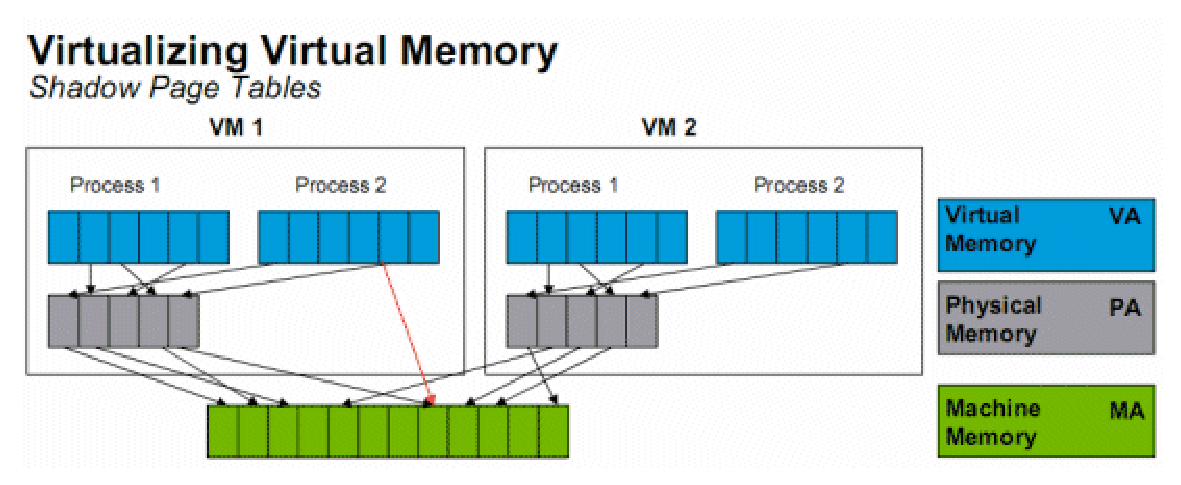
\includegraphics[width=0.7\textwidth]{images/allocmodel}
        	%\caption[Page Table Illustration]{Illustration of \textit{VA} $\rightarrow$ \textit{PA} address translation.}
    		\captionsource{Virtualized Physical Memory Allocation Model}{Physical memory allocation model in virtualized systems.}%
    		{\url{images.anandtech.com/reviews/it/2008/virtualization-nuts-bolts/Shadowpt.gif}}  
    \label{fig:allocmodel}
     \end{center}
\end{figure}

\section{Techniques of Virtualizing the MMU} \label{techniques}
This section discusses how the hypervisor defines ways for the guest OS to access the actual
machine frames through the MMU functionalities provided by it.\\
We know that the guest OS maintains page table related information for every process running in a
VM and also that the guest OS operates on pseudo physical pages or GPFNs. Memory references by
processes running in a VM  requires translation of virtual addresses into machine addresses via
hardware MMU operations such as page table walk. The page table walk itself needs actual machine
frames addresses to get to the different levels of page table as discussed in \ref{native}. But as
discussed in \ref{challenges} the guest OS cannot be given unrestricted direct access to the
machine frames holding the page table pages to ensure VM isolation. This means that the guest OS
access to the actual MMU (or its functionalities) in the VMM, like CR3 access, changes to page
table entries need to be supervised by the VMM.\\
Table \ref{tab:tech} lists the existing methodologies of virtualizing MMU.
\begin{table}[tbp]
  \begin{center}
    \caption{MMU virtualization techniques.}
    \label{tab:tech}
    \begin{tabular}{ll}
      \toprule 
      Technique & Description \\
      \midrule
      Shadow Paging & Software approach\\
      Direct Paging &  Para-virtualization approach\\
      Nested Page Tables & Hardware assisted approach\\
      \bottomrule \\
    \end{tabular}
  \end{center}
\end{table}
\subsection{Shadow Paging} \label{sp}
Shadow paging mechanism is a software MMU virtualization mechanism.
The access to CR3 is by default protected by design paradigms of virtualization which pushed the
guest OS to lower privilege levels than the hypervisor. The machine frames that contain the
different page table levels are protected by making them write protected. And for each
process in a VM, just like a guest OS maintains a page table, the hypervisor also maintains a page
table called the \textit{Shadow Page Table}. The shadow page table is part of a plan to easily get
the direct the V $\rightarrow$ M mapping instead of going through \textit{V} $\rightarrow$
\textit{P} and then \textit{P} $\rightarrow$ \textit{M} as mentioned in \ref{model}. Ideally every
virtual address that is translated to corresponding guest physical page address in the guest OS
should be translated to the corresponding machine frame address via P $\rightarrow$ M in the VMM.
This applies to guest physical page addresses that correspond to the pages of the guest OS page
table as well. But there is a subtle drawback to this approach. To translate a virtual address we
know that the guest OS needs to access the page table whose base address is stored in the CR3.
Assuming we have access to the CR3, for the time being, can we go ahead and directly access the
guest page table? No, because what the guest OS have is only the guest physical page address of
the the page table base. What we need is the address of the machine frame that holds this guest
physical page. And in order to access it we need to do a translation using the P $\rightarrow$ M
mappings. This needs to be repeated for the base address of every level of the page table.\\
In order to alleviate this overhead we make use of the same P $\rightarrow$ M mappings maintained
by the VMM for a VM to create shadow page tables for all process that run in that VM. And in
the shadow page tables we maintain the direct V $\rightarrow$ M mappings. Thus every virtual
address access by a process in a VM can now go through the corresponding shadow page table in the
VMM saving on the number of memory accesses and the corresponding latency. Figure
\ref{fig:shadowpagetables} illustrates this.\\
\begin{figure}[tbp]
  \begin{center}
    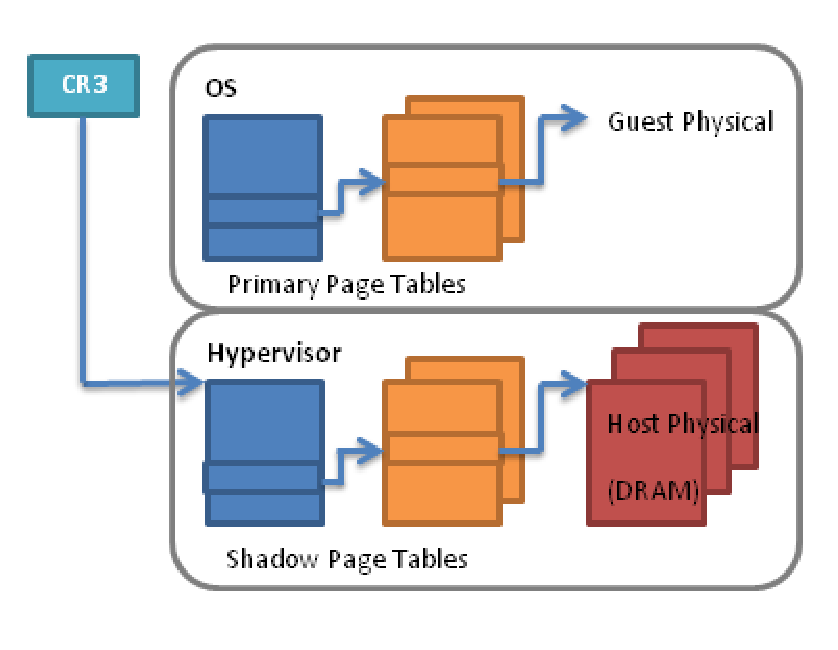
\includegraphics[width=0.7\textwidth]{images/shadowpagetables}
        	%\caption[Page Table Illustration]{Illustration of \textit{VA} $\rightarrow$ \textit{PA} address translation.}
        	\captionsource{Shadow Page Table Illustration}{Shadow Page Table Illustration.}{\url{corensic.files.wordpress.com/2011/12/shadowpagetables.png}}  
    \label{fig:shadowpagetables}
     \end{center}
\end{figure}
To pull off this trick the guest OS's CR3 is virtualized and guest OS access to the CR3 is to be
prevented by a general protection fault (GPF) \citep{wiki1}. The VMM should load the CR3 with the
base address of the shadow page table rather than with the base of guest OS page table. Virtual
memory access that reads or writes already mapped frames can go ahead via the shadow page table
unhindered. When a page fault occurs the VMM checks if the guest page table has valid entries for
the faluting address, if that is the case then fault occurred because the VMM had moved the
machine frame corresponding to the faulting address to its swap space. This type of fault should
be hidden from the guest OS as such a fault would not have occurred if the guest OS was running on
a native system. The VMM now swaps in the contents of the faulting address into machine memory,
updates the P $\rightarrow$ M mapping to reflect this and the updates the corresponding shadow
page table. On the other hand if the fault occurred because the guest page table did not have
valid mappings for this virtual address, the VMM transfers control to the trap handler of the
guest indicating a page fault. The guest OS will then issues I/O requests to effect a page-in
operation, which may or may not cause a dirty page swap out. These requests are in fact serviced
by the VMM as they are privileged instructions. Once the guest physical page (and the machine
frame backing it is) is available the guest OS issues instructions to the modify the guest page
tables \citep{smith2005virtual}. This causes an exception called \textbf{VMExit} as the frames
containing guest page tables are write protected from the guest OS. The VMM now updates the guest
page table and the mappings in the shadow page table before returning control back to the guest.
This is done to ensure that the shadow page table is in sync with the guest page table.  
\subsection{Direct Paging} \label{para}
Direct Paging uses an approach called \textit{Para-Virtualization} in which the guest OS
is made aware of being virtualized. Guest OS is modified as a part of the MMU virtualization. This
approach makes use of the \textbf{VMCALL} or \textit{hypercall} API provided by para-
virtualization. This is a solution to the x86 architecture virtualization issue. More
can be read from \citet{force2000analysis}.\\
The major change that this brings about is in the way in which guest page tables are updated.
There is no shadow page table in this approach. Here also the machine frames containing the guest
page tables are write protected by making them read only. A change to the guest page table are
carried out by a VMCALL from the guets OS to the VMM. Subsequently the VMM VMCALL handler carries
out the changes to the corresponding machine frames after validating them to ensure isolation.
Hence the guest page tables contains direct \textit{virtual address} $\rightarrow$ \textit{machine
address} mappings that are VMM validated. As it is the case with shadow paging mechanism
normal page table reads happen without VMM intervention and page faults are handled by the guest
OS by updating the page table entries through the VMM. Figure \ref{fig:para} illustrates this
approach.
\begin{figure}[tbp]
  \begin{center}
    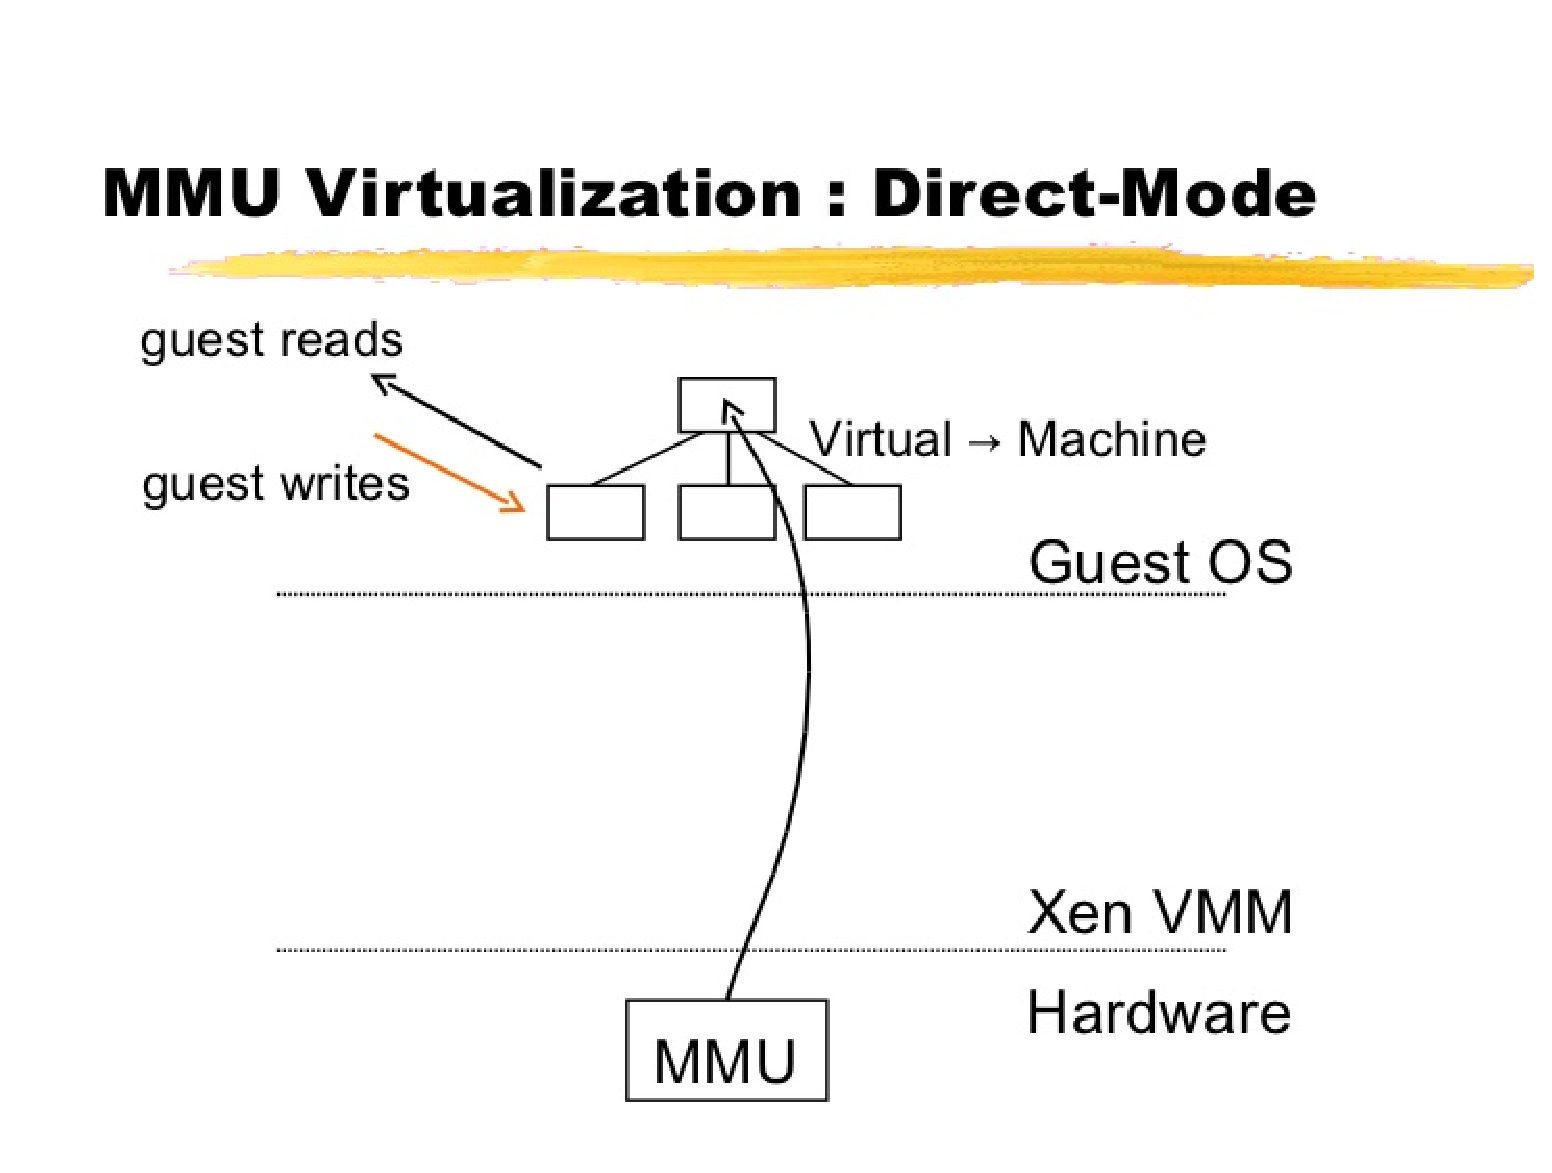
\includegraphics[width=0.7\textwidth]{images/paravirt}
        	%\caption[Page Table Illustration]{Illustration of \textit{VA} $\rightarrow$ \textit{PA} address translation.}
        	\captionsource{Direct Mapping Illustration}{Direct Mapping Illustration.}{\url{image.slidesharecdn.com/overview-of-xen-30627/95/overview-of-xen-30-12-728.jpg}}  
    \label{fig:para}
     \end{center}
\end{figure}
\subsection{Nested Page Tables} \label{nested}
Extensions to the hardware in the form \textit{extended page tables or nested page tables} (EPT or
NPT) enabled a new mechanism to achieve memory virtualization called \textit{hardware assisted MMU
virtualization}. Contrary to shadow paging, nested paging removes the need for the VMM to
supervise the guest OS page table operations once the nested pages are populated. Under nested
paging both guest and the hypervisor have their own copy of the CR3 register. The guest OS maps
virtual addresses to guest physical addresses and the Nested page tables (NPT) map guest physical
addresses to machine frame addresses. The guest now is allowed to set up the guest page tables
without any hindrance (i.e VMExits) by the VMM, except for getting a physical frame allocated (for
the guest page table or any other guest physical page) which is still under the preview of the
VMM. The VMM sets up the nested page table. A guest OS virtual memory reference, when nested page
tables are set up, results in a 2-D page table walk - first in the guest page table and next in
the nested page table - to get to the corresponding machine frame. Parts of virtual address is
used to index into the guest page tables, as explain in \ref{native}, to obtain the guest physical
address and using this guest physical address we do a similar indexing into the nested page table
to obtain the machine frame address. There is a subtle issue here that may miss our eyes easily.
While translating a virtual address we need to access machine frames holding the guest page table
pages, so for each level of guest page table accessed we need to do a nested page table walk to
reach the machine frame holding this page table page.\\
If the guest page tables contain \textit{n levels} and the nested page table contains \textit{m
levels}, then to resolve a virtual address to corresponding machine frame we require \[((n+1)\ *\
m) + n\] memory accesses. For getting the machine frame address of a particular level of guest
page table physical page we need to traverse \textbf{n} levels of nested page table. Once the
machine frame is identified we need 1 memory access for reading it. These are the \textbf{n + 1}
memory accesses in the previous expression. This is repeated for all levels of guest page table.
Hence the \textbf{(n+1) * m}. Once you reach the machine frame which holds the last level of guest
page table i.e. the PTE machine frame you can read the guest physical address of the original
virtual address address and finally to obtain its machine address we need to traverse the nested
page tables one last time. That is why the \textbf{n} term is added to the equation.
This is illustrated in figure \ref{fig:npt}.\\
\begin{figure}[tbp]
  \begin{center}
    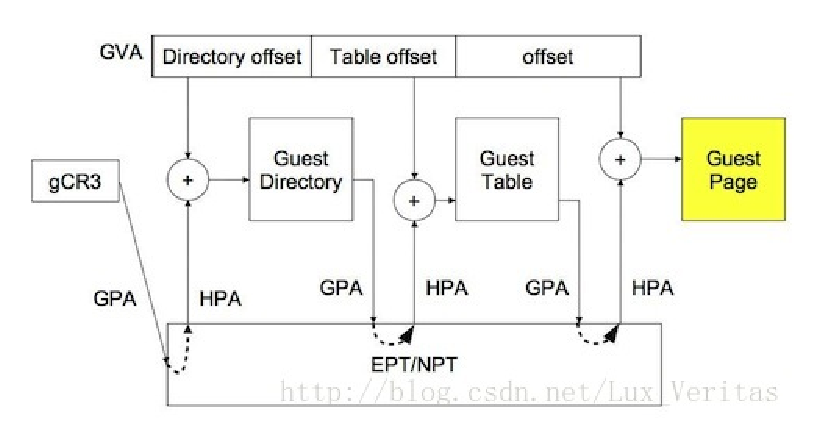
\includegraphics[width=0.7\textwidth]{images/npt}
        	%\caption[Page Table Illustration]{Illustration of \textit{VA} $\rightarrow$ \textit{PA} address translation.}
        	\captionsource{Nested Page Table Illustration}{Nested Page Table Illustration.}{\url{cnblogs.com/snake-hand/p/3181631.html}}  
    \label{fig:npt}
     \end{center}
\end{figure}

\section{Comparison of Memory Virtualization Techniques}
Following table compares the different memory virtualization techniques.
\begin{table}[!htbp]
  \begin{center}
    \caption{Comparing Memory Virtualization Techniques.}
    \label{tab:compare}
    \begin{tabular}{p{3cm} p{5cm} p{5cm}}
      \toprule 
      Technique & Advantage & Disadvantage \\
      \midrule
      Shadow Paging & Software approach, no changes to guest OS  & Frequent costly VMExits for each guest page table updation.\\
      \midrule
      Direct Paging &  No VMExits & Requires changes to the guest OS.\\
      \midrule
      Nested Page Tables & Hardware assisted approach, No VMExits, No changes to guest OS. & More number of memory for a virtual memory translation. About 6 times more. \\
      \bottomrule \\
    \end{tabular}
  \end{center}
\end{table}
\section{Optimizations to Memory Virtualization Techniques}
Shadow Paging and Nested Page Tables are two approaches that doesn't require changes to the guest
OS. The solution approach they take, though seems similar, are independent of each other. If a 
process running in the guest OS is experiencing large number of page faults then shadow paging is
going to degrade the performance because of frequent VMExits required to synchronize the guest and
shadow page tables (refer \ref{sp}). Hence shadow paging will prove to be a bad memory
virtualization technique for such a process. Now consider another scenario where a process is
experiencing large number of TLB misses but its pages are still in memory i.e. it has few page
faults, then resolving their machine address by doing a 2-D page table walk in nested paging
mechanism is going to degrade its performance due to increased number of memory accesses (refer
\ref{nested}). For this process nested paging proves to be a bad choice of memory virtualization
technique.
\subsection{Combining Shadow Paging \& Nested Page Table}
Neither of the two strategies is a clear winner all the time for different mix of processes
possible in a VM. Hence in order to get the best of these two techniques \citet{wang2011selective}
proposes a dynamic switching mechanism that switches between the shadow paging and nested paging
based on memory access behaviour of the VMs and they call it the \textit{Dynamic Switching Paging}
or DSP. Their solution approach is as follows:
\begin{itemize}
\item Determine page fault frequency and TLB miss frequency measured as the number of page faults
and the number of TLB misses per thousand retired (finished) instructions.
\item Determine system dependent upper and lower thresholds for page faults frequency \& TLB miss
frequency.
\item If one metric is beyond its upper threshold \& the other is well within within its threshold
limits, then switch to the technique/mode that is the most suitable for the metric that is within
its limits.
\begin{itemize}
\item ``If the TLB miss frequency is higher than the TLB miss upper-bound threshold and the page
fault frequency is lower than 80 percent of the page fault upper-bound threshold, switch from''
nested page table mode to shadow page table mode or stay in shadow page table mode if already in
it.
\item ``If the page fault frequency is higher than the page fault upper-bound threshold and the
TLB miss frequency is lower than 80 percent of the TLB miss upper-bound threshold, switch from''
shadow paging mode to nested page table mode or stay in nested page table mode if already in it.  
\end{itemize}
\item If both metrics are below their lower threshold limits then remain in the current mode. 
\item If both metrics are above their upper threshold values or within their threshold limits find
out the relative penalty between them.
\item Calculate the relative penalty as the P-to-T ratio. \[P-to-T ratio\ =\ \frac{Page\ Fault\ 
Frequency}{TLB\ Miss\ Frequency}\]
\item P-to-T ratio is used along with a running average of recent P-to-T ratios called historic P-
o-T ratios.
\item If either of historic TLB miss frequency or current TLB miss frequency is zero then switch
from shadow paging to nested page tables without estimating either historic or current P-to-T
ratio. This avoids divide by zero errors.
\item If both historic and latest P-to-T ratio are above P-to-T ratio threshold upper bound switch
from shadow paging to nested page tables or stay in nested page tables if already in it.
\item If both historic and latest P-to-T ratio are lower than P-to-T ratio threshold lower bound
switch from nested page tables to shadow paging or stay in shadow paging mode if already in it.
\item If both historic and latest P-to-T ratio are within the P-to-T ratio threshold's lower \&
upper bounds stay in current mode.
\item If historic and latest P-to-T ratio falls into different threshold intervals, a clear trend
cannot be estimated and hence it is better to stay back in current mode.     
\end{itemize}
Through experimentations they claim that DSP is capable of matching the performance of the better
among shadow paging and nested page tables, though they do not explain clearly how they attributed
the performance degradation of particular processes to the memory virtualization technique used.
\subsection{Reducing the number of Memory Accesses while using Nested Page Table}     
The advantages of nested Page table technique make it a good memory virtualization technique. But
its drawback of large number of memory access for a single virtual address translation is too much
of a cost for processes having poor memory access locality. \citet{gandhi2014efficient} proposes
new hardware that makes use of \textit{Direct Segments} both in the guest OS and the hypervisor to
reduce the overhead of virtualized address translation. The concept of direct segments is
explained in \citet{basu2013efficient}. They incorporate the idea presented there to introduce
virtualized direct segments that logically reside on the TLB miss path of the guest OS and on the
address translation mechanism used in the VMM. Direct segments maps a processes virtual address
space with segments and with paging. This enables large parts of contiguous virtual address space
to be mapped to contiguous physical addresses with minimal hardware. And for portions that cannot
be contiguously mapped direct segments fall back on normal paging. As with normal memory
management with \textit{egements} rather than pages, in native systems, which we did not discuss
in section \ref{introduction}, direct segments are also managed with 3 registers: BASE, LIMIT and
OFFSET. As we know a virtual address V within a segment ($BASE\ \leq\ V\ \leq LIMIT$) gets
translated to physical address $V\ +\ OFFSET$. The contiguous address space required for the
segment is obtained by mapping a large chunk of contiguous virtual addresses with the same
permissions, which is called the \textit{primary region} abstraction in \citet{basu2013efficient}.  
\\
The different modes of operation that they propose are the following:
\begin{itemize}
\item \textit{Dual Direct} mode that uses direct segments both in the guest OS and VMM. It uses
the direct segment registers both in the guest OS and VMM to translate directly from \textit{guest
virtual address} $\rightarrow$ \textit{machine address}, thus bypassing both dimensions of
virtualized address translation. 
\item \textit{VMM Direct Mode} uses direct segments for the 2nd dimension of virtualized address
translation i.e. \textit{guest physical address} $\rightarrow$ \textit{machine address}. Hence the
guest OS can be left unmodified. Only the VMM needs modifications to support this mode.
\item \textit{Guest Direct} mode limits the support of direct segments to the guest OS.
\textit{guest virtual address} $\rightarrow$ \textit{guest physical address} translations now has
zero overhead. VMM uses normal paging techniques to manage the actual machine memory. 
\end{itemize} 
In effect they flatten one or two dimensions of the page walk based on the mode of operation. They also address the possibility of lack of contiguous guest physical memory needed to create a direct segment due to fragmentation using \textit{self ballooning}. Self ballooning uses \textit{ballooning} to remove the fragmented guest physical memory form use and \textit{hotplug} it back as contiguous guest physical memory that can be used to create guest direct segments. They also talk about plugging gaps caused by faulty pages in the contiguous direct segments by using \textit{escape filters}. Escape filters are nothing but making use of conventional paging to map holes in the physical address that break the addresses' physical contiguity. Hence while using direct segments and translating addresses, along with the segment register we need too check the hardware that implements the filter to \textit{escape} the faulty page from segment based translation to paging.     